\section{Trimmed regions and the witness}
\label{sec:regions}

The lower bound and the trimming come from one object, the distance between the sets of kernel mean embeddings that
the trimmings of two laws produce. This section defines it and shows that the two sets first meet at the contamination
level, that in every direction each set reaches exactly as far as a trimmed mean, and that the direction of the
difference of their closest points selects the trimming. The last two facts, and the empirical regions as polytopes, are RKHS
forms of known properties of zonoid trimmed regions and reduced convex hulls, and the equivalence \eqref{eq:zeroeq}
follows at once from \eqref{eq:tvintersect} for a characteristic kernel. New are the uniform concentration
\eqref{eq:hausdorff} and the analysis of the path in Section~\ref{sec:rates}.

\subsection{Trimmings and total variation}

We observe $X_1,\dots,X_n$ i.i.d.\ $P$ and $Y_1,\dots,Y_m$ i.i.d.\ $Q$, two independent samples on a measurable space
$\mathcal X$, with empirical measures $P_n$ and $Q_m$; we write $u_+=\max(u,0)$, $a\vee b=\max(a,b)$ and
$a\wedge b=\min(a,b)$. For $0\le\alpha<1$ let $\beta=(1-\alpha)^{-1}$. Formally, the \emph{$\alpha$-trimmings} of $P$ are the laws
\begin{equation}
R_\alpha(P)\coloneqq\Big\{P'\ll P:\ \frac{dP'}{dP}\le\beta\ \ P\text{-almost surely}\Big\}.
\label{eq:trimset}
\end{equation}
This trimming is impartial, in that the data decide what is removed, with no region such as the tails prescribed
\citep{gordaliza1991best,cuesta1997trimmed}. The fact of \citet{alvarez2012similarity} recalled in the introduction reads
\begin{equation}
\TV(P,Q)\le\alpha
\iff
R_\alpha(P)\cap R_\alpha(Q)\neq\varnothing ,
\label{eq:tvintersect}
\end{equation}
or, equivalently, there are probability measures $R$, $P_0$ and $Q_0$ with
\begin{equation}
P=(1-\alpha)R+\alpha P_0,
\qquad
Q=(1-\alpha)R+\alpha Q_0 ,
\label{eq:contam}
\end{equation}
and from now on $\alpha^\star\coloneqq\TV(P,Q)$ always denotes the contamination level of the pair at hand. At
$\alpha^\star$ the common component is the \emph{common core} $R^\star=(P\wedge Q)/(1-\alpha^\star)$, where $P\wedge Q$ has density $\min(p,q)$ for
densities $p$ and $q$ of $P$ and $Q$ with respect to any common dominating measure. Its complement $1-\alpha^\star$ is the overlapping
coefficient of $P$ and $Q$ \citep{inman1989overlapping}. For instance, if $P$ puts mass $\tfrac12$ on each of two
points $x_1,x_2$ and $Q$ on each of $x_2,x_3$, then $\alpha^\star=\tfrac12$, and removing $x_1$ from $P$ and $x_3$
from $Q$ leaves the point mass at $x_2$ in both. The level is shared because both laws lose the same fraction. If
they lose fractions $\alpha_1$ and $\alpha_2$ and what remains coincides, then $\alpha_1\vee\alpha_2\ge\alpha^\star$
(Section~\ref{app:regions} of the supplement).

The kernel $k$ on $\mathcal X$ has reproducing kernel Hilbert space (RKHS) $\Hh$ and feature map
$\phi(x)=k(x,\cdot)$, so that $f(x)=\langle f,\phi(x)\rangle_\Hh$ for $f\in\Hh$, and as in the introduction
$\mu_P=\E_P[\phi(X)]$ and $\MMD(P,Q)=\|\mu_P-\mu_Q\|_\Hh$ \citep{gretton2012kernel,muandet2017kernel}. Two constants of the kernel
enter our bounds, $\kappa=\sup_xk(x,x)^{1/2}$, which bounds the norm of every feature vector, and the diameter
$\Delta_\phi=\sup_{x,x'}\|\phi(x)-\phi(x')\|_\Hh\le2\kappa$ of the feature vectors. The Laplace kernel
$k(x,y)=\exp(-\|x-y\|/\sigma)$ and the Gaussian kernel $k(x,y)=\exp(-\|x-y\|^2/(2\sigma^2))$ on $\R^d$, of bandwidth $\sigma$, both have
$\kappa=1$ and $\Delta_\phi=\sqrt2$, and Section~\ref{sec:numerical} says where each is used.

\begin{assumption}
\label{ass:regularity}
$\mathcal X$ is a measurable space, with no further structure. Moreover:
\begin{enumerate}[label=(A\arabic*),leftmargin=*]
\item $x\mapsto k(x,x')$ is measurable for every $x'$, and $k(x,x)\le\kappa^2$ for all $x$;
\item $\Hh$ is separable;
\item $k$ is characteristic, that is, $\MMD(P',Q')=0$ only if $P'=Q'$, for probability measures $P',Q'$ on
$\mathcal X$ \citep{sriperumbudur2010hilbert}.
\end{enumerate}
\end{assumption}

Assumption~\ref{ass:regularity} holds for the Gaussian, Laplace and inverse multiquadric kernels on $\R^d$, and for
any bounded continuous characteristic kernel on a separable metric space, so curves, or graphs with a characteristic
kernel, are covered on the same terms as vectors. Theorem~\ref{thm:plugin} uses only (A1) and (A2),
Theorem~\ref{thm:betting} needs only that the function bet on be measurable with values in $[0,1]$, and (A3) makes the
split-sample bound consistent (Proposition~\ref{prop:loconsistency}).

\subsection{Trimmed regions}

The \emph{trimmed maximum mean discrepancy} is
\begin{equation}
D_\alpha(P,Q)\coloneqq\inf\big\{\MMD(P',Q'):\ P'\in R_\alpha(P),\ Q'\in R_\alpha(Q)\big\} ,
\label{eq:trimMMDpop}
\end{equation}
an analogue of optimal partial transport \citep{caffarelli2010free,figalli2010partial} with the MMD between the kept
parts in place of a transport cost, and with the Wasserstein distance the outlier-robust distance of
\citet{nietert2022robust}. \citet{mukherjee2021robust} penalize the change made to one law, kernel mean matching
\citep{huang2007correcting,gretton2008covariate} reweights one sample toward the other, and robust MMD estimators
\citep{lerasle2019monk,cherief2022finite} protect against a contamination, where we measure it. The \emph{trimmed
region} of $P$ is
\begin{equation}
\mathcal C_\alpha(P)\coloneqq\big\{\E_P[g(X)\phi(X)]:\ 0\le g\le\beta,\ \E_P[g(X)]=1\big\}\subset\Hh ,
\label{eq:region}
\end{equation}
the set of kernel mean embeddings of all $\alpha$-trimmings of $P$, since $g$ ranges over their densities. The regions
grow with $\alpha$ from the single point $\mu_P$, and Figure~\ref{fig:regions} draws them for two laws on three
points. For sets $A,B\subset\Hh$ we write $\dist(A,B)=\inf\{\|a-b\|_\Hh:\ a\in A,\ b\in B\}$, and
$\dist(a,B)=\dist(\{a\},B)$.

\begin{proposition}[Geometric representation]
\label{prop:georep}
Under Assumption~\ref{ass:regularity}, for every $\alpha\in[0,1)$,
\begin{equation}
D_\alpha(P,Q)=\dist\big(\mathcal C_\alpha(P),\mathcal C_\alpha(Q)\big),
\label{eq:setdist}
\end{equation}
and $\mathcal C_\alpha(P_n)=\{\sum_iw_i\phi(X_i):\ 0\le w_i\le\beta/n,\ \sum_iw_i=1\}$ is a polytope.
\end{proposition}

\begin{lemma}[Compactness and attainment]
\label{lem:attainment}
Under Assumption~\ref{ass:regularity}, $\mathcal C_\alpha(P)$ is convex, norm-bounded by $\kappa$ and
norm-compact. Hence the infimum in \eqref{eq:trimMMDpop} is attained at trimmings $P^\star\in R_\alpha(P)$ and
$Q^\star\in R_\alpha(Q)$, and if $D_\alpha(P,Q)=0$, then $\mathcal C_\alpha(P)\cap\mathcal C_\alpha(Q)$ is nonempty and
each of its elements is the embedding of a common trimming $R\in R_\alpha(P)\cap R_\alpha(Q)$.
\end{lemma}

With \eqref{eq:tvintersect} and (A3), these two results give
\begin{equation}
D_\alpha(P,Q)=0\iff\TV(P,Q)\le\alpha .
\label{eq:zeroeq}
\end{equation}
We call
$\alpha\mapsto D_\alpha(P,Q)$ the \emph{population path} of the trimmed distance, and its empirical counterpart
$\alpha\mapsto\widehat D_\alpha$ of Section~\ref{sec:statistic} the \emph{empirical path}. The population path is
positive below $\alpha^\star$ and zero from $\alpha^\star$ on, as in the right panel of Figure~\ref{fig:regions}. It
is nonincreasing, because the regions are nested, and Lipschitz with constant $4\kappa/(1-\bar\alpha)^2$ on
$[0,\bar\alpha]$ for every $\bar\alpha<1$ (Lemma~\ref{lem:continuity} of the supplement).

\begin{figure}[t]
\centering
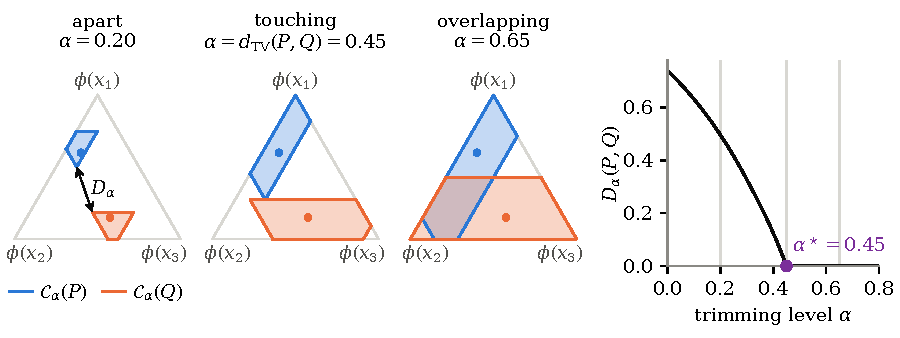
\includegraphics[width=\textwidth]{figs_print/fig0_regions.pdf}
\caption{Left: the regions $\mathcal C_\alpha(P)$ and $\mathcal C_\alpha(Q)$ of laws with weights $(\regWeightsP)$ and
$(\regWeightsQ)$ on three points whose feature vectors are unit vectors at $120$ degrees in the plane, drawn
isometrically (untrimmed embeddings as dots), at $\alpha=\regAlphaLo$, at $\alpha=\TV(P,Q)=\regTV$ and at
$\alpha=\regAlphaHi$. Right: the distance $D_\alpha(P,Q)$, computed exactly, with these levels marked.}
\label{fig:regions}
\end{figure}

A closed convex set $A\subset\Hh$ is determined by its support function $h_A(f)=\sup_{a\in A}\langle a,f\rangle_\Hh$,
how far it reaches in the direction $f$. For the trimmed regions this function is a familiar risk measure, the
conditional value-at-risk of finance \citep{rockafellaruryasev2000}.

\begin{lemma}[Support function]
\label{lem:cvar}
Under Assumption~\ref{ass:regularity}, for every $f\in\Hh$,
\begin{equation}
h_{\mathcal C_\alpha(P)}(f)
=\sup_{0\le g\le\beta,\ \E_Pg=1}\E_P[g(X)f(X)]
=\inf_{t\in\R}\Big\{t+\beta\,\E_P\big[(f(X)-t)_+\big]\Big\},
\label{eq:cvar}
\end{equation}
the supremum is attained, and the second equality holds for every bounded measurable $f$.
\end{lemma}

The first equality is the reproducing property, and the right-hand side is the representation by
\citet{rockafellaruryasev2000} of the mean of $f(X)$ over the upper $(1-\alpha)$-fraction of its distribution, an atom
at the cut being split. The lemma is the RKHS instance of the defining property of zonoid trimmed regions
\citep{koshevoy1997zonoid,dyckerhoff2011weighted}.

Maximizing $\E_P[gf]$ over trimming densities is a bathtub problem, whose solution $g$ fills its cap $\beta$ on the
largest values of $f$ until the mass runs out and is zero below. In a fixed direction the optimal trimming therefore
keeps the part of the law on one side of a cut, the level set $\{f\ge t\}$ with $t$ the $\alpha$-quantile of $f(X)$,
and the minimizing $t$ in \eqref{eq:cvar} is that cut.

For each fixed $t$, moreover, the expression inside the infimum is an ordinary mean, of the bounded function
$t+\beta(f-t)_+$. A region is thus a family of trimmed means, one per direction, and a trimmed mean is an infimum of
ordinary means. Means of bounded functions, and of bounded vectors of $\Hh$, concentrate at the rate $n^{-1/2}$ with
constants that depend only on the bound $\kappa$, and this rate cannot be improved for the mean embedding or the MMD
\citep{tolstikhin2016minimax,tolstikhin2017minimax}. Every finite-sample validity statement below reduces to such
means, and the empirical regions are uniformly close to the population ones,
\begin{equation}
\sup_{0\le\alpha<1}(1-\alpha)\,d_H\big(\mathcal C_\alpha(P_n),\mathcal C_\alpha(P)\big)
\le\kappa\Big[\frac4{\sqrt n}+\sqrt{\frac{2\log(2/\delta)}n}\,\Big]
\label{eq:hausdorff}
\end{equation}
with probability at least $1-\delta$, for every $P$, where $d_H$ is the Hausdorff distance in $\Hh$
(Corollary~\ref{cor:uniform} of the supplement). No complexity of the sample space enters \eqref{eq:hausdorff}, because the
regions live in $\Hh$ and the kernel bound $\kappa$ is their only constant.

\subsection{The statistic, its witness and the trimming it selects}
\label{sec:statistic}

The statistic is $\widehat D_\alpha\coloneqq D_\alpha(P_n,Q_m)$, and $\alpha\mapsto\widehat D_\alpha$ is the empirical
path. By Proposition~\ref{prop:georep} it is the distance between two polytopes, the square root of
\begin{equation}
\widehat D_\alpha^{\,2}
=\min_{w,v}\big\{w^\top K_{XX}w+v^\top K_{YY}v-2w^\top K_{XY}v\big\}
\label{eq:qp}
\end{equation}
over the capped simplices $0\le w_i\le\beta/n$, $\sum_iw_i=1$ and $0\le v_j\le\beta/m$, $\sum_jv_j=1$, where $K_{XX}$,
$K_{YY}$ and $K_{XY}$ are the Gram matrices. The objective is $\|\sum_iw_i\phi(X_i)-\sum_jv_j\phi(Y_j)\|_\Hh^2$, so
\eqref{eq:qp} is a convex quadratic program, the problem of the nearest points of two reduced convex hulls, which is the
dual of the $\nu$-support vector machine \citep{bennett2000duality,crisp1999geometric,takeda2008nusvm}. The witness
below is the normal of its hyperplane, and Proposition~\ref{prop:bangbang} is the structure of its support vectors read
as a trimming. We solve it by accelerated projected gradient (Section~\ref{sec:computationdetails} of the supplement). For a minimizer $(w,v)$, the \emph{witness}, the name that \citet{gretton2012kernel} use at $\alpha=0$, is
the difference of the two closest points,
\begin{equation}
\widehat d=\sum_iw_i\phi(X_i)-\sum_jv_j\phi(Y_j),
\qquad
\widehat d(x)=\sum_iw_ik(X_i,x)-\sum_jv_jk(Y_j,x).
\label{eq:witness}
\end{equation}
It is a function on $\mathcal X$, large where the trimmed first sample has more mass than the trimmed second, and it
can be evaluated at points not used to compute it. Its direction $\widehat f=\widehat d/\widehat D_\alpha$, with $\widehat f=0$ when $\widehat D_\alpha=0$,
separates the two empirical regions. The population witness $d^\star$ is the element of minimal norm of
$\mathcal C_\alpha(P)-\mathcal C_\alpha(Q)$, with direction $f^\star=d^\star/D_\alpha(P,Q)$.

Let $\mathcal T_\alpha$ be the set of minimizers $(w,v)$ of \eqref{eq:qp}. Each of them is a pair of trimmed samples,
since the weighted empirical measures $P_n^w=\sum_iw_i\delta_{X_i}$ and $Q_m^v=\sum_jv_j\delta_{Y_j}$ are
$\alpha$-trimmings of $P_n$ and $Q_m$ whose embeddings are at distance $\widehat D_\alpha$. The witness determines
them.

\begin{proposition}[Structure of the empirical trimming]
\label{prop:bangbang}
The set $\mathcal T_\alpha$ is nonempty, convex and compact. Moreover:
\begin{enumerate}[label=(\roman*),leftmargin=*]
\item the difference $\widehat d=\sum_iw_i\phi(X_i)-\sum_jv_j\phi(Y_j)$ takes the same value at every
$(w,v)\in\mathcal T_\alpha$, namely the element of minimal norm of $\mathcal C_\alpha(P_n)-\mathcal C_\alpha(Q_m)$, and
$\|\widehat d\|_\Hh=\widehat D_\alpha$;
\item if $\widehat D_\alpha>0$, let $n_{1-\alpha}=\lfloor n(1-\alpha)\rfloor$ and let $\widehat t_n$ be the
$(n_{1-\alpha}+1)$-th smallest of the values $\widehat d(X_1),\dots,\widehat d(X_n)$, with $\widehat t_n=+\infty$ if
$n_{1-\alpha}=n$. Then every $(w,v)\in\mathcal T_\alpha$ has $w_i=\beta/n$ when $\widehat d(X_i)<\widehat t_n$ and $w_i=0$
when $\widehat d(X_i)>\widehat t_n$, the observations with $\widehat d(X_i)=\widehat t_n$ sharing the remaining mass.
Symmetrically, with $m_{1-\alpha}=\lfloor m(1-\alpha)\rfloor$, $v_j=\beta/m$ when $\widehat d(Y_j)$ is above the
$(m_{1-\alpha}+1)$-th largest of the values $\widehat d(Y_1),\dots,\widehat d(Y_m)$, $v_j=0$ when it is below, and the ties
share the remainder;
\item if $\widehat D_\alpha=0$, then $\mathcal T_\alpha$ is the set of all feasible $(w,v)$ with
$\sum_iw_i\phi(X_i)=\sum_jv_j\phi(Y_j)$.
\end{enumerate}
\end{proposition}

Part (ii) is the bathtub of Lemma~\ref{lem:cvar} in the direction of the witness. Once $\widehat d$ is fixed the
problem is linear: the weights on the $X$'s minimize $\sum_iw_i\widehat d(X_i)$ over the capped simplex, and those on
the $Y$'s maximize $\sum_jv_j\widehat d(Y_j)$. So every optimal trimming of the first sample keeps at full weight the
observations on which the witness is smallest, the most $Q$-like ones, discards those above the cut and splits weight
only among ties at the cut, and the trimming of the second sample is the level set above a cut of the same function.
The cuts reappear in the betting test of Section~\ref{sec:split}. Part (iii) does not arise for $\alpha<1$ with a
strictly positive definite kernel and pairwise distinct pooled observations $X_1,\dots,X_n,Y_1,\dots,Y_m$, since the
feature vectors are then linearly independent and the minimizer is unique. Many observations may still share the cut,
as support vectors share the margin of a $\nu$-support vector machine, and with the Laplace kernel on the line all the
$X$'s whose witness values have rank $\lceil n(1-\alpha)\rceil$ or higher share it (Lemma~\ref{lem:lapclip} of the
supplement). For kernels whose empirical regions can meet we return the minimizer closest to uniform
weights (Section~\ref{sec:computationdetails} of the supplement).

\subsection{No informative upper bound}
\label{sec:upper}

By \eqref{eq:zeroeq}, $\TV(P,Q)>\alpha$ exactly when the regions are apart, and Sections~\ref{sec:analytic}
and~\ref{sec:split} certify this by lower confidence bounds valid on any sample space. We certify only from below
because no upper confidence bound on $\TV(P,Q)$ can be valid for all pairs of laws and still informative, as
\citet[Theorem~1.1]{horebarber2026blurred} prove for $\TV$ and \citet[Theorem~9]{blanchard2010semi} for mixture
proportions, in a line that goes back to \citet{bahadursavage1956} and \citet{donoho1988onesided}. The version below
holds even for laws on $[0,1]$ with densities bounded by $2$, and its conclusion is at $P=Q$.

\begin{theorem}[No informative upper bound, even for bounded densities]
\label{thm:impossible}
Fix $n,m\ge1$ and $\delta\in(0,1)$, and let $\mathcal P_2$ be the set of pairs of probability measures on $[0,1]$
whose densities with respect to Lebesgue measure are bounded by $2$. Suppose that
$\widehat U=\widehat U(X_{1:n},Y_{1:m})$, measurable and possibly randomized, satisfies
$\Pp_{P,Q}(\TV(P,Q)\le\widehat U)\ge1-\delta$ for every $(P,Q)\in\mathcal P_2$. Then, with $P_{\mathrm u}$ the uniform
law on $[0,1]$, $\Pp_{P_{\mathrm u},P_{\mathrm u}}(\widehat U\ge1)\ge1-\delta$.
\end{theorem}

A fixed kernel is blind in the same way: densities that oscillate ever faster stay at total variation $\tfrac12$ from
the uniform law while their MMD to it tends to zero (Section~\ref{sec:upperimposs} of the supplement). An upper end
needs an assumption, such as a margin with known constants, since $D_\alpha(P,Q)\ge c_0(\alpha^\star-\alpha)^\gamma$
gives $\alpha^\star\le\alpha+(\check D_\alpha/c_0)^{1/\gamma}$ for any $\check D_\alpha\ge D_\alpha(P,Q)$, or a blurred
version of $\TV$, and the data do not identify $c_0$ and $\gamma$. Lower bounds escape the argument, because rejecting
$\TV(P,Q)\le\alpha$ needs only one set on which the samples differ, but their rates do not: a valid lower bound with a
rate uniform over $\mathcal P_2$ would give an informative upper bound, so some restriction such as the margin is needed
for any rate.
